\documentclass{article}
\usepackage{graphicx}
\usepackage{subfigure}
\usepackage{fullpage}
\usepackage{verbatim}
\usepackage{amsmath}
\usepackage{tikz}
\usepackage{listings}

\begin{document}
\title{Example for the ICSE'13 paper}
\maketitle

Figure~\ref{partialOutput} with the code on the left and its CFG on the middle left demonstrates two static data-flow analyses. The result of the {\em zero} analysis (with the abstract domain elements $0$ and $\neg 0$) is on the middle left . The results of the {\em sign} analysis (with the abstract domain elements $-$, $0$ and $+$) is on the right. 

We can see none of the analysis able to determine that $\phi$ holds, thus the analyses cannot be compared in term of their usefulness. However, the {\em sign} analysis reports two infeasible branches: the true branch of the second x$>$0 conditional statement and the true branch of y$==$0. While {\em zero} analysis only able to detect that the true outcome of y$==0$ is infeasible. Therefore using the partial information obtained from the analyses we can conclude that {\em sign} analysis has better fit. 

Obviously there is no surprise there since the abstract domain of the {\em sing} analysis is ``finer'' then the abstract domain of the {\em zero} analysis. The point we want to make  is that partial information can be used to evaluate the fit between analyses to a program.

Figure~\ref{partialAnalysis} demonstrates the result of partial {\em zero} analysis for different controlling/restricting mechanism. The result of the left of Figure~\ref{partialAnalysis} shows what happens if we restrict the input value of x$_{in}$ to zero. In this case the {\em zero} analysis was able to verify that the property holds. The result on the middle shoes the attempt of the analysis to evaluate the program on the input x$_{in}=\neg 0$, i.e., on another ``half'' of the input domain. However, as in its full version the analysis is not able to verify the program (in this case only the result different from the full version is shown). 

The result on the right of Figure~\ref{partialAnalysis} depicts the case when the set of paths that the analysis considers is explicitly restricted to follow the true branch of the first conditional statement. In this case the analysis also proves that for all feasible and infeasible paths that traverse the true outcome of the first conditional statement the property is not violated. (Of course, this information might imply to explore paths for non-zero input values of x$_{in}$ that explore the false branch of x$>$0, but his is not what the paper is about). 

But it might not always be the case that using the restriction an analysis can decide $\phi$. Thus partial information can be used to answer the research question, i.e., what type of control, i.e., predicate-based, path-based or their combination, produces more partial output. (It might also be the case that the result of a partial weaker analysis is comparable with the results of full stronger analysis, but once again this comparison is not in the objectives of this paper.)

\begin{figure*}[t]
\begin{minipage}{0.22\textwidth}
\small
\begin{lstlisting}
if (x > 0){
  y = x;
  x = 0; 
} 

if(x > 0){
  x = -x;
} else if (y == 0){
  x = 1;
}
assert(x == 0);
\end{lstlisting}
\end{minipage}
~
\begin{minipage}{0.22\textwidth}
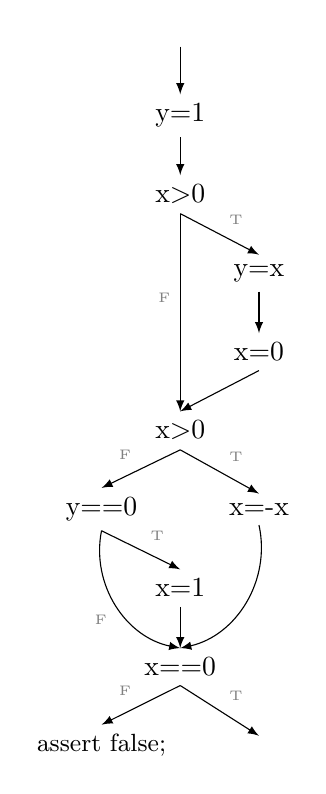
\begin{tikzpicture}[>=latex]
\node[name=enter]{};
\node[name=stmt_1, below of=enter]{y=1};
\node[name=if_1, below of=stmt_1]{x$>$0};
\node[name=if_1_body_1, below of=if_1, xshift=10mm]{y=x};
\node[name=if_1_body_2, below of=if_1_body_1]{x=0};
\node[name=if_2, below of=if_1_body_2, xshift=-10mm]{x$>$0};
\node[name=if_2_true, below of=if_2, xshift=10mm]{x=-x};
\node[name=if_3, below of=if_2, xshift=-10mm]{y==0};
\node[name=if_3_true, below of=if_3, xshift=10mm]{x=1};
\node[name=assert, below of=if_3_true]{x==0};
\node[name=exit, below of=assert, xshift=10mm] {};
\node[name=assertFalse, below of=assert, xshift=-10mm] {\small assert false;};

\draw(enter.south) edge[->](stmt_1.north);
\draw(stmt_1.south) edge[->](if_1.north);
\draw(if_1.south) edge[->]node[above right]{\tiny {\color{gray}T}}(if_1_body_1.north);
\draw(if_1_body_1.south) edge[->](if_1_body_2.north);
\draw(if_1_body_2.south) edge[->](if_2.north);
\draw(if_1.south) edge[->]node[above left]{\tiny {\color{gray}F}}(if_2.north);
\draw(if_2.south) edge[->]node[above right]{\tiny {\color{gray}T}}(if_2_true.north);
\draw(if_2.south) edge[->]node[above left]{\tiny {\color{gray}F}}(if_3.north);
\draw(if_3.south) edge[->]node[above right]{\tiny {\color{gray}T}}(if_3_true.north);
\draw(if_3_true.south) edge[->](assert.north);
\draw(if_3.south) edge[->, bend right=45]node[below left]{\tiny {\color{gray}F}}(assert.north);
\draw(if_2_true.south) edge[->, bend right=-45](assert.north);
\draw(assert.south) edge[->]node[above left]{\tiny {\color{gray}F}}(assertFalse.north);
\draw(assert.south) edge[->]node[above right]{\tiny {\color{gray}T}}(exit.north);

\end{tikzpicture}
\end{minipage}
~
\begin{minipage}{0.22\textwidth}
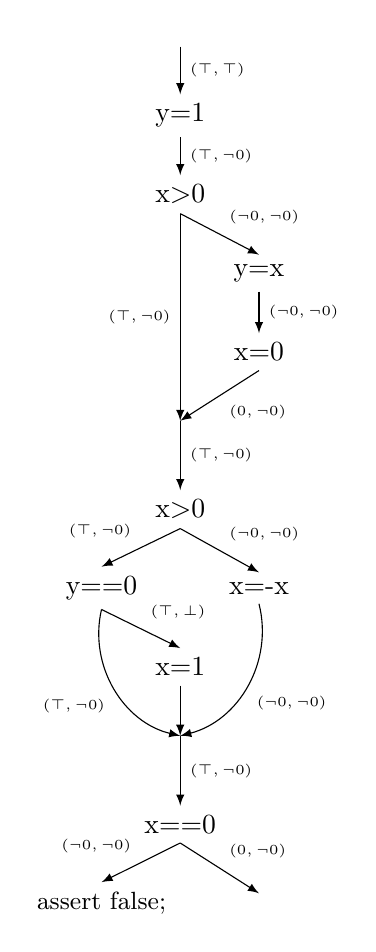
\begin{tikzpicture}[>=latex]
\node[name=enter]{};
\node[name=stmt_1, below of=enter]{y=1};
\node[name=if_1, below of=stmt_1]{x$>$0};
\node[name=if_1_body_1, below of=if_1, xshift=10mm]{y=x};
\node[name=if_1_body_2, below of=if_1_body_1]{x=0};
\node[name=if_1_merge, below of=if_1_body_2, xshift=-10mm]{};
\node[name=if_2, below of=if_1_merge]{x$>$0};
\node[name=if_2_true, below of=if_2, xshift=10mm]{x=-x};
\node[name=if_3, below of=if_2, xshift=-10mm]{y==0};
\node[name=if_3_true, below of=if_3, xshift=10mm]{x=1};
\node[name=if_2_merge, below of=if_3_true]{};
\node[name=assert, below of=if_2_merge]{x==0};
\node[name=exit, below of=assert, xshift=10mm] {};
\node[name=assertFalse, below of=assert, xshift=-10mm] {\small assert false;};

\draw(enter.south) edge[->]node[right]{\tiny $(\top,\top)$}(stmt_1.north);
\draw(stmt_1.south) edge[->]node[right]{\tiny $(\top,\neg 0)$}(if_1.north);
\draw(if_1.south) edge[->]node[above right]{\tiny $(\neg 0, \neg 0)$}(if_1_body_1.north);
\draw(if_1_body_1.south) edge[->]node[right]{\tiny $(\neg 0,\neg 0)$}(if_1_body_2.north);
\draw(if_1_body_2.south) edge[->]node[below right]{\tiny $(0,\neg 0)$}(if_1_merge.north);
\draw(if_1.south) edge[->]node[left]{\tiny $(\top,\neg 0)$}(if_1_merge.north);
\draw(if_1_merge.north) edge[->]node[right]{\tiny $(\top, \neg 0)$}(if_2.north);
\draw(if_2.south) edge[->]node[above right]{\tiny $(\neg 0, \neg 0)$}(if_2_true.north);
\draw(if_2.south) edge[->]node[above left]{\tiny $(\top,\neg 0)$}(if_3.north);
\draw(if_3.south) edge[->]node[above right]{\tiny $(\top, \bot)$}(if_3_true.north);
\draw(if_3_true.south) edge[->](if_2_merge.north);
\draw(if_3.south) edge[->, bend right=45]node[below left]{\tiny $(\top, \neg 0)$}(if_2_merge.north);
\draw(if_2_true.south) edge[->, bend right=-45]node[below right]{\tiny $(\neg 0, \neg 0)$}(if_2_merge.north);
\draw(if_2_merge.north) edge[->]node[right]{\tiny $(\top,\neg 0)$}(assert.north);
\draw(assert.south) edge[->]node[above left]{\tiny $(\neg 0, \neg 0)$}(assertFalse.north);
\draw(assert.south) edge[->]node[above right]{\tiny $(0, \neg 0)$}(exit.north);
\end{tikzpicture}
\end{minipage}
~
\begin{minipage}{0.22\textwidth}
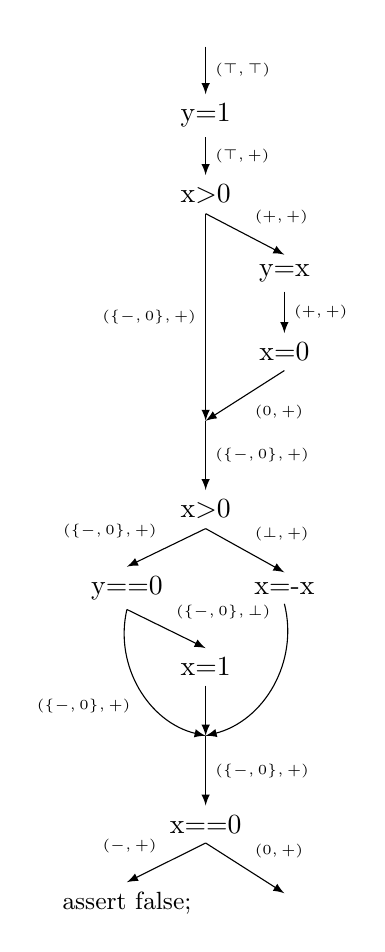
\begin{tikzpicture}[>=latex]
\node[name=enter]{};
\node[name=stmt_1, below of=enter]{y=1};
\node[name=if_1, below of=stmt_1]{x$>$0};
\node[name=if_1_body_1, below of=if_1, xshift=10mm]{y=x};
\node[name=if_1_body_2, below of=if_1_body_1]{x=0};
\node[name=if_1_merge, below of=if_1_body_2, xshift=-10mm]{};
\node[name=if_2, below of=if_1_merge]{x$>$0};
\node[name=if_2_true, below of=if_2, xshift=10mm]{x=-x};
\node[name=if_3, below of=if_2, xshift=-10mm]{y==0};
\node[name=if_3_true, below of=if_3, xshift=10mm]{x=1};
\node[name=if_2_merge, below of=if_3_true]{};
\node[name=assert, below of=if_2_merge]{x==0};
\node[name=exit, below of=assert, xshift=10mm] {};
\node[name=assertFalse, below of=assert, xshift=-10mm] {\small assert false;};

\draw(enter.south) edge[->]node[right]{\tiny $(\top,\top)$}(stmt_1.north);
\draw(stmt_1.south) edge[->]node[right]{\tiny $(\top,+)$}(if_1.north);
\draw(if_1.south) edge[->]node[above right]{\tiny $(+,+)$}(if_1_body_1.north);
\draw(if_1_body_1.south) edge[->]node[right]{\tiny $(+,+)$}(if_1_body_2.north);
\draw(if_1_body_2.south) edge[->]node[below right]{\tiny $(0,+)$}(if_1_merge.north);
\draw(if_1.south) edge[->]node[left]{\tiny $(\{-,0\},+)$}(if_1_merge.north);
\draw(if_1_merge.north) edge[->]node[right]{\tiny $(\{-,0\},+)$}(if_2.north);
\draw(if_2.south) edge[->]node[above right]{\tiny $(\bot, +)$}(if_2_true.north);
\draw(if_2.south) edge[->]node[above left]{\tiny $(\{-,0\},+)$}(if_3.north);
\draw(if_3.south) edge[->]node[above right]{\tiny $(\{-,0\}, \bot)$}(if_3_true.north);
\draw(if_3_true.south) edge[->](if_2_merge.north);
\draw(if_3.south) edge[->, bend right=45]node[below left]{\tiny $(\{-,0\}, +)$}(if_2_merge.north);
\draw(if_2_true.south) edge[->, bend right=-45](if_2_merge.north);
\draw(if_2_merge.north) edge[->]node[right]{\tiny $(\{-,0\},+)$}(assert.north);
\draw(assert.south) edge[->]node[above left]{\tiny $(-,+)$}(assertFalse.north);
\draw(assert.south) edge[->]node[above right]{\tiny $(0,+)$}(exit.north);
\end{tikzpicture}
\end{minipage}
\caption{Partial output example: source code (left), CFG (middle left), the zero analysis result (middle right), and the sign analysis result (right).} 
\label{partialOutput}
\end{figure*}

\begin{figure*}[t]
\begin{minipage}{0.30\textwidth}
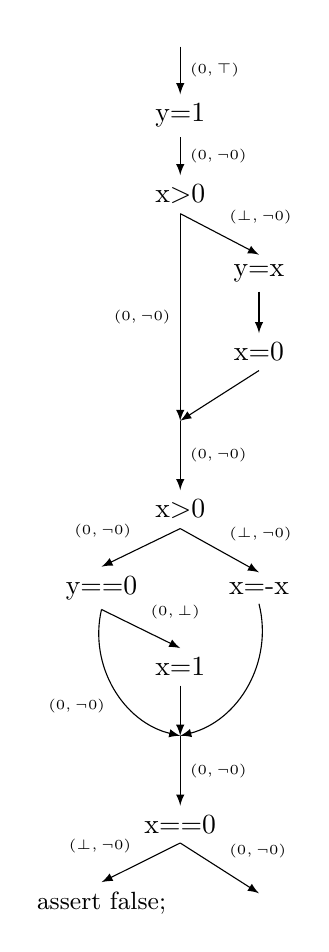
\begin{tikzpicture}[>=latex]
\node[name=enter]{};
\node[name=stmt_1, below of=enter]{y=1};
\node[name=if_1, below of=stmt_1]{x$>$0};
\node[name=if_1_body_1, below of=if_1, xshift=10mm]{y=x};
\node[name=if_1_body_2, below of=if_1_body_1]{x=0};
\node[name=if_1_merge, below of=if_1_body_2, xshift=-10mm]{};
\node[name=if_2, below of=if_1_merge]{x$>$0};
\node[name=if_2_true, below of=if_2, xshift=10mm]{x=-x};
\node[name=if_3, below of=if_2, xshift=-10mm]{y==0};
\node[name=if_3_true, below of=if_3, xshift=10mm]{x=1};
\node[name=if_2_merge, below of=if_3_true]{};
\node[name=assert, below of=if_2_merge]{x==0};
\node[name=exit, below of=assert, xshift=10mm] {};
\node[name=assertFalse, below of=assert, xshift=-10mm] {\small assert false;};

\draw(enter.south) edge[->]node[right]{\tiny $(0,\top)$}(stmt_1.north);
\draw(stmt_1.south) edge[->]node[right]{\tiny $(0,\neg 0)$}(if_1.north);
\draw(if_1.south) edge[->]node[above right]{\tiny $(\bot, \neg 0)$}(if_1_body_1.north);
\draw(if_1_body_1.south) edge[->](if_1_body_2.north);
\draw(if_1_body_2.south) edge[->](if_1_merge.north);
\draw(if_1.south) edge[->]node[left]{\tiny $(0,\neg 0)$}(if_1_merge.north);
\draw(if_1_merge.north) edge[->]node[right]{\tiny $(0, \neg 0)$}(if_2.north);
\draw(if_2.south) edge[->]node[above right]{\tiny $(\bot, \neg 0)$}(if_2_true.north);
\draw(if_2.south) edge[->]node[above left]{\tiny $(0,\neg 0)$}(if_3.north);
\draw(if_3.south) edge[->]node[above right]{\tiny $(0, \bot)$}(if_3_true.north);
\draw(if_3_true.south) edge[->](if_2_merge.north);
\draw(if_3.south) edge[->, bend right=45]node[below left]{\tiny $(0, \neg 0)$}(if_2_merge.north);
\draw(if_2_true.south) edge[->, bend right=-45](if_2_merge.north);
\draw(if_2_merge.north) edge[->]node[right]{\tiny $(0,\neg 0)$}(assert.north);
\draw(assert.south) edge[->]node[above left]{\tiny $(\bot, \neg 0)$}(assertFalse.north);
\draw(assert.south) edge[->]node[above right]{\tiny $(0, \neg 0)$}(exit.north);
\end{tikzpicture}
\end{minipage}
~
\begin{minipage}{0.30\textwidth}
\begin{tikzpicture}[>=latex]
\node[name=enter]{};
\node[name=stmt_1, below of=enter]{y=1};
\node[name=if_1, below of=stmt_1]{x$>$0};
\node[name=if_1_body_1, below of=if_1, xshift=10mm]{y=x};
\node[name=if_1_body_2, below of=if_1_body_1]{x=0};
\node[name=if_1_merge, below of=if_1_body_2, xshift=-10mm]{};
\node[name=if_2, below of=if_1_merge]{x$>$0};
\node[name=if_2_true, below of=if_2, xshift=10mm]{};
\node[name=if_3, below of=if_2, xshift=-10mm]{};
\node[name=if_3_true, below of=if_3, xshift=10mm]{};
\node[name=if_2_merge, below of=if_3_true]{};
\node[name=assert, below of=if_2_merge]{};
\node[name=exit, below of=assert, xshift=10mm] {};
\node[name=assertFalse, below of=assert, xshift=-10mm] {};

\draw(enter.south) edge[->]node[right]{\tiny $(\neg 0,\top)$}(stmt_1.north);
\draw(stmt_1.south) edge[->]node[right]{\tiny $(\neg 0,\neg 0)$}(if_1.north);
\draw(if_1.south) edge[->]node[above right]{\tiny $(\neg 0, \neg 0)$}(if_1_body_1.north);
\draw(if_1_body_1.south) edge[->]node[right]{\tiny $(\neg 0, \neg 0)$}(if_1_body_2.north);
\draw(if_1_body_2.south) edge[->]node[below right]{\tiny $(0, \neg 0)$}(if_1_merge.north);
\draw(if_1.south) edge[->]node[left]{\tiny $(\neg 0,\neg 0)$}(if_1_merge.north);
\draw(if_1_merge.north) edge[->]node[right]{\tiny $(\top, \neg 0)$}(if_2.north);

\end{tikzpicture}
\end{minipage}
~
\begin{minipage}{0.30\textwidth}
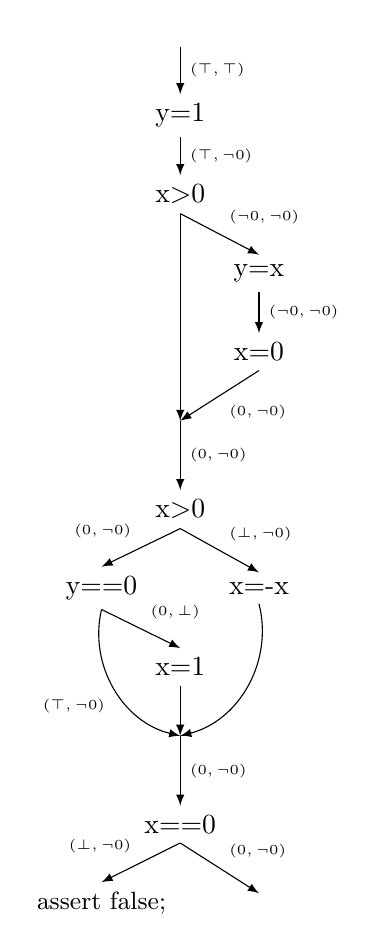
\begin{tikzpicture}[>=latex]
\node[name=enter]{};
\node[name=stmt_1, below of=enter]{y=1};
\node[name=if_1, below of=stmt_1]{x$>$0};
\node[name=if_1_body_1, below of=if_1, xshift=10mm]{y=x};
\node[name=if_1_body_2, below of=if_1_body_1]{x=0};
\node[name=if_1_merge, below of=if_1_body_2, xshift=-10mm]{};
\node[name=if_2, below of=if_1_merge]{x$>$0};
\node[name=if_2_true, below of=if_2, xshift=10mm]{x=-x};
\node[name=if_3, below of=if_2, xshift=-10mm]{y==0};
\node[name=if_3_true, below of=if_3, xshift=10mm]{x=1};
\node[name=if_2_merge, below of=if_3_true]{};
\node[name=assert, below of=if_2_merge]{x==0};
\node[name=exit, below of=assert, xshift=10mm] {};
\node[name=assertFalse, below of=assert, xshift=-10mm] {\small assert false;};

\draw(enter.south) edge[->]node[right]{\tiny $(\top,\top)$}(stmt_1.north);
\draw(stmt_1.south) edge[->]node[right]{\tiny $(\top,\neg 0)$}(if_1.north);
\draw(if_1.south) edge[->]node[above right]{\tiny $(\neg 0, \neg 0)$}(if_1_body_1.north);
\draw(if_1_body_1.south) edge[->]node[right]{\tiny $(\neg 0,\neg 0)$}(if_1_body_2.north);
\draw(if_1_body_2.south) edge[->]node[below right]{\tiny $(0,\neg 0)$}(if_1_merge.north);
\draw(if_1.south) edge[->](if_1_merge.north);
\draw(if_1_merge.north) edge[->]node[right]{\tiny $(0, \neg 0)$}(if_2.north);
\draw(if_2.south) edge[->]node[above right]{\tiny $(\bot, \neg 0)$}(if_2_true.north);
\draw(if_2.south) edge[->]node[above left]{\tiny $(0,\neg 0)$}(if_3.north);
\draw(if_3.south) edge[->]node[above right]{\tiny $(0, \bot)$}(if_3_true.north);
\draw(if_3_true.south) edge[->](if_2_merge.north);
\draw(if_3.south) edge[->, bend right=45]node[below left]{\tiny $(\top, \neg 0)$}(if_2_merge.north);
\draw(if_2_true.south) edge[->, bend right=-45](if_2_merge.north);
\draw(if_2_merge.north) edge[->]node[right]{\tiny $(0,\neg 0)$}(assert.north);
\draw(assert.south) edge[->]node[above left]{\tiny $(\bot, \neg 0)$}(assertFalse.north);
\draw(assert.south) edge[->]node[above right]{\tiny $(0, \neg 0)$}(exit.north);
\end{tikzpicture}
\end{minipage}
\caption{Partial zero analysis example: predicate-based restriction x$_{in}=$0 (left), predicate-based restriction x$_{in}=$!0 (middle), path-based restriction the true branch of x$>$0  by the path (right).} 
\label{partialAnalysis}
\end{figure*}

\end{document}